\documentclass[10pt]{article}

\usepackage{subfiles}
\usepackage{hyperref}

\usepackage[utf8]{inputenc}
\usepackage[toc]{appendix}
\usepackage[swedish]{babel}
\usepackage[margin=2cm]{geometry}
\usepackage{graphicx}
\usepackage{scrextend}
\usepackage[backend=bibtex,sorting=none,style=numeric,natbib=true]{biblatex}
\usepackage{filecontents}
\usepackage{enumitem}

\usepackage[section]{placeins}

\usepackage{xifthen}
\usepackage{enumitem}
\usepackage{scrextend}
\newcounter{switchcase}

\newcommand{\ifequals}[3]{\ifthenelse{\equal{#1}{#2}}{\stepcounter{switchcase} #3}{}}
\newcommand{\case}[2]{#1 #2} % Dummy, so \renewcommand has something to overwrite...
\newenvironment{switch}[1]{
  %Executed at \begin{switch}
  \setcounter{switchcase}{0}
  \renewcommand{\case}{\ifequals{#1}}
}{
 % Executed at \end{switch}
\ifthenelse{\equal{\value{switchcase}}{0}}{
  \PackageError{ProjectDefinitions}{Could not find given definition}{}}{}
}

\newcommand{\definition}[1]
{
  \begin{switch}{#1}
    \case{Cachning}{\item [\textbf{#1}]
      Temporär lagning av data för snabb åtkomst.}
    \case{Instans}{\item [\textbf{#1}]
      En spelsession som startas från UI-applikationen och spelare kan gå med i för att spela spelet tillsammans.}
    \case{IoT-backend}{\item [\textbf{#1}]
      Existerande system som kan dirigera data mellan många uppkopplade enheter.}
    \case{Kontroll-applikation}{\item [\textbf{#1}]
      Applikation som körs på en mobil eller surfplatta och tar input från användare.}
    \case{Progressive Web Apps}{\item [\textbf{#1}]
      Förkortat PWA, är ett mellanting mellan en hemsida och en applikation.
      Med en PWA behöver man inte ladda ner en app, men den ger viss funktionalitet som appar har. \cite{bib-pwa}}
    \case{Resurs}{\item [\textbf{#1}]
      Media som används i spelet, t.ex. bilder och ljud.}
    \case{Sensor}{\item [\textbf{#1}]
      En sensor som sitter på kontroll-applikationen och inte är en pekskärm, t.ex. en accelerometer.}
    \case{Server-klient-modell}{\item [\textbf{#1}]
      Struktur på ett system där någon enhet tillhandahåller resurser, information eller tjänster och flera andra enheter interagerar med denna.}
    \case{Spelläge}{\item [\textbf{#1}]
      En utökning av grundspelet som definierar speciella regler och spelmekanik.}
    \case{Spelmekanik}{\item [\textbf{#1}]
      Regler och möjligheter som definierar ett spel.}
    \case{Tunn klient}{\item [\textbf{#1}]
      Specialfall av server-klient-modell där mycket få beräkningar sker på klienten.}
    \case{UI-applikation}{\item [\textbf{#1}]
      Applikationen som kör spelet och visar spelplanen.}
    \case{Use Case Map}{\item [\textbf{#1}]
      Diagram som illustrerar hur olika händelser interagerar med arkitekturen. \cite[p.~30--33]{bib-architecture-primer}}
    \case{Scrum-board}{\item [\textbf{#1}]
      En tavla med post-it lappar som innehåller aktiviteter som ska göras under
      projektet. Detta komplementeras med olika kolumner i tavlan såsom planerad, pågående,
      testning och utgåva. Dessa bestämmer i vilket stadie lapparna befinner sig i.}
    \case{Burndown-chart}{\item [\textbf{#1}]
      En graf som visar hur många timmar medlemmarna har lagt ner i förhållande till vad som krävs för att hinna med projektet.}
    \case{Acceptanstest}{\item [\textbf{#1}]
      Slutgiltiga testet som kund utför för att se att produkten lever upp till förväntningarna.}
    \case{Enhetstest}{\item [\textbf{#1}]
      Testa varje enhet så den fungerar när den är färdig.}
    \case{Integrationstest}{\item [\textbf{#1}]
      Testa att en ny enhet som läggs till i projektet fungerar som den ska tillsammans med de andra enheterna.}
    \case{Kund}{\item [\textbf{#1}]
      Cybercom Sweden.}
    \case{Regressionstest}{\item [\textbf{#1}]
      Testa ny kod enligt gamla parametrar för att säkerställa att ingen funktionalitet försvunnit.}
    \case{Systemtest}{\item [\textbf{#1}]
      Test för att säkerställa att enheten uppfyller kraven för projektet.}
    \case{Cybercom}{\item [\textbf{#1}]
      Kortare variant av Cybercom Sweden, företaget produkten utvecklas åt.}
    \case{Enkäten}{\item [\textbf{#1}]
      Den enkät som ska användas för att utvärdera användarupplevelsen, se avsnitt  3.3 Demo och enkät.}
    \case{Kvalitet}{\item [\textbf{#1}]
        I likhet med IEEE 730 definierar denna rapport kvalitet som konformitet till projektets krav. \cite{ieee730}}
    \case{Projektet}{\item [\textbf{#1}]
        Processen att framställa en produkt åt Cybercom Sweden.}
    \case{Software Quality Asssurance}{\item [\textbf{#1}]
    	Förkortat SQA, är en samling aktiviteter som bedömmer lämpligheten och inger förtroende
    	för utvecklingsmetodiken som används.}
    \case{SQA-process}{\item [\textbf{#1}]
      I likhet med IEEE 730 definieras en SQA-process som aktiviteten att samla underlag för att med säkerhet ta
      beslutet av produkten uppnår sina kvalitetskrav}
    \case{Teamet}{\item [\textbf{#1}]
      Det team av åtta studenter som tillsammans ska utföra projektet}
    \case{Trello}{\item [\textbf{#1}]
      En hemsida för att lägga till och fördela uppgifter bland flera personer, kan liknas till en whiteboard som
      postit lappar fästs på.}
    \case{Speldata}{\item [\textbf{#1}]
      Information om handlingar och status i spelet samt nödvändig teknisk data för
      att upprätthålla kommunikation.}
    \case{Realtidsmultiplayerspel}{\item [\textbf{#1}]
      Spel där flera användares handlingar har en direkt inverkan på spelets tillstånd.}
    \case{Gamemode}{\item [\textbf{#1}]
      En variant av basspelet med eventuellt andra funktioner och regler.}
    \case{Vanliga nätverksförhållanden}{\item [\textbf{#1}]
      En enhet med en stabil internetuppkoppling utan yttre störningar.}
    \case{React}{\item [\textbf{#1}]
      Javascript-bibliotek för att bygga hemsidor och mer avancerade webbsystem.\cite{bib-react}}
    \case{Deep Stream}{\item [\textbf{#1}]
    Kommunikationssystem som tillåter synkronisering av data mellan många enheter i realtid. Tillgängligt i många olika programmeringsspråk, bland annat javascript.\cite{bib-deepstream}}
    \case{Impact Map}{\item [\textbf{#1}]
    Diagram som visar inverkan av händelser under ett mjukvarusystems livstid. Kan visa på effekterna av implementation av ny funktionalitet, fel i systemet eller säkerhetsintrång.\cite[p.~91--93]{bib-architecture-primer}}
    \case{IoT, Internet of things}{\item [\textbf{#1}]
    Internet of things -- Ett begrepp som beskriver den tekniska och samhälleliga utveckling då fler och fler saker blir uppkopplade mot internet.}
    \case{Gitrepo}{\item [\textbf{#1}]
    En datastruktur för att lagra och hantera olika versioner av kod i git.}
    \case{Master-branch}{\item [\textbf{#1}]
    Standardgrenen till ett gitrepo som vanligtvis reflekterar repot i ett fungerande tillstånd.}
	\case{Kursen}{\item [\textbf{#1}]
    Den kurs som detta projekt utförs inom, det vill säga LiTHs kurs ''Kandidatprojekt i programvaruutveckling'' med kurskod TDDD96}
  \case{npm}{\item [\textbf{#1}]
  Node Package Manager -- En pakethanterare för Javascripts ekosystem}
  \case{npm-paket}{\item [\textbf{#1}]
  Ett paket med Javascript-kod som finns tillängligt i npm}


  \end{switch}
}


%Skriv över engelska namn för appendix
\addto\captionsswedish{
  \renewcommand\appendixname{Appendix}
  \renewcommand\appendixpagename{Appendix}
	\renewcommand\appendixtocname{Appendix}
}

\newcommand{\History}[3]{
	\centering #1 & #2 & #3 \\ \hline
}

\graphicspath{ {images/} }
\selectlanguage{swedish}
\addbibresource{../references.bib}

\tolerance=1
\emergencystretch=\maxdimen
\hyphenpenalty=10000
\hbadness=10000

\setlength{\parindent}{0pt}

\begin{document}
    \pagenumbering{gobble}
		\title{Projektplan\\
    \large Projektgrupp 1}

\author{
    Joel Almqvist\\
    \texttt{xxxxxxxx@student.liu.se}
    \and
    Björn Detterfelt\\
    \texttt{xxxxxxxx@student.liu.se}
    \and
    Tim Håkansson\\
    \texttt{timha404@student.liu.se}
    \and
    David Kjellström\\
    \texttt{xxxxxxxx@student.liu.se}
    \and
    Axel Löjdquist\\
    \texttt{xxxxxxxx@student.liu.se}
    \and
    Joel Oskarsson\\
    \texttt{joeos014@student.liu.se}
    \and
    Lieth Wahid\\
    \texttt{xxxxxxxx@student.liu.se}
    \and
    Alexander Wilkens\\
    \texttt{xxxxxxxx@student.liu.se}
}

\date{Februari 19, 2018}

\maketitle
\pagebreak

		\pagebreak
    \section*{Dokumenthistorik}

\begin{center}
    \begin{tabular}{| l | l | p{12cm} |}
        \hline
        \textbf{Version} & \textbf{Datum} & \textbf{Förändring och kommentar} \\ \hline
        \History{1.0}{2018-02-19}{Första inlämningen}
        \History{2.0}{2018-02-19}{Andra inlämningen, ändringar baserat på respons från inlämning 1.}
    \end{tabular}
\end{center}

    \pagebreak

		\tableofcontents
    \pagebreak
		\listoffigures
		\pagebreak

    \pagenumbering{arabic}
		\section{Inledning}
Arkitektursbeskrivningen står till grund för strukturen hos ett system. Den ska underlätta implementationen genom att ge en översiktlig bild över olika komponenter och hur de interagerar. Arkitekturen är även central för uppfyllandet av både funktionella krav och kvalitetskrav.\\

Det system som detta dokument beskriver är ett realtids-spel som tjänar till syfte att demonstrera ett existerande system för kommunikation mellan enheter. Den arkitektur som beskrivs är till stor del baserad på en server-klient-modell. Den innehåller dock en central komponent, IoT-backend, som gör att arkitekturen får en något annorlunda struktur jämfört med traditionella implementationer av denna modell.\\

Detta dokument innehåller förutom modeller över arkitekturen även den bakomliggande motivering som har gjort att arkitekturen ser ut som den gör. Arkitekturen finns representerade på olika abstraktionsnivåer och ur olika perspektiv. Modeller åtföljs även av beskrivningar och återkoppling till hur modellen förhåller sig till motiveringen. I dokumentet presenteras även en diskussion kring problem, risker och eventuella utökningar av arkitekturen.\\

		\pagebreak

    \section{Definitioner}
\begin{itemize}[leftmargin=3cm]
  \item [Cachning] Temporär lagning av data för snabb åtkomst
  \item [Instans] En spelsession som startas från UI-applikationen och spelare kan gå med i för att spela spelet tillsammans
  \item [IoT-backend] Existerande system som kan dirigera data mellan många uppkopplade enheter
  \item [Kontroll-applikation] Applikation som körs på en mobil eller surfplatta och styr spelet
  \item [Progressive Web Apps] Ett mellanting mellan en hemsida och en applikation. Med en PWA behöver man inte ladda ner en app, men den ger viss funktionalitet som appar har. \cite{bib-pwa}
  \item [Resurs] Media som används i spelet, t.ex. bilder och ljud
  \item [Sensor] En sensor som sitter på kontroll-applikationen och inte är en pekskärm, t.ex. en accelerometer
  \item [Server-klient-modell] Struktur på ett system där någon enhet tillhandahåller resurser, information eller tjänster och flera andra enheter interagerar med denna
  \item [Spelläge] En utökning av grundspelet som definierar speciella regler och spelmekanik
  \item [Spelmekanik] Regler och möjligheter som definierar ett spel
  \item [Tunn klient] Specialfall av server-klient-modell där mycket få beräkningar sker på klienten
  \item [UI-applikation] Applikationen som kör själva spelet och visar upp spelplanen
  \item [Use Case Map] Diagram som illustrerar hur olika händelser interagerar med arkitekturen \cite[p.~30--33]{bib-architecture-primer}
\end{itemize}

		\pagebreak

		\section{Motivering}
I denna del listas de krav och mål som påverkar systemets arkitektur. Specifika krav, centrala kvalitetsaspekter och andra viktiga faktorer i systemet får direkta eller indirekta konsekvenser för arkitekturen. Dessa har legat till grund för uppdelningen av systemet i komponenter och definitionen av kommunikationen mellan dem.

\subsection{Arkitekturkritiska Krav}
Kraven återfinns i dokumentet kravspecifikation \cite{bib-kravspec}. Notera att samtliga krav ej har konsekvenser för arkitekturen.\\

\begin{center}
    \begin{tabular}{|p{1cm}|p{13cm}|}
        \hline
        \textbf{Nr} & \textbf{Arkitekturella konsekvenser}\\
        \hline
        1 & Då prestandan på enheten som kör kontroll-applikationen är begränsad bör arkitekturen för denna hållas enkel och liten. Kontroll-applikationen bör efterlikna en tunn klient.\\
        \hline
        3 & UI-Applikationen bör kunna lägga till spelare utan att det stör spelets flöde.\\
        \hline
        4 & Delen av systemet som finns på IoT-backenden måste hantera och identifiera olika instanser av UI-Applikationen.\\
        \hline
        5 & En komponent för att generera och hantera de olika identifikationskoderna bör existera.\\
        \hline
        8 & En komponent för att visa upp ett grafiskt gränssnitt bör finnas i kontroll-applikationen.\\
        \hline
        18 & För att klara av flera klienter är det bra om kommunikationen i UI-applikationen sker på en robust, specialiserad komponent.\\
        \hline
        21 & All speldata som går ut från UI-applikationen bör gå genom ett gemensamt gränssnitt.\\
        \hline
        25, 26 & Programspråket Javascript sätter vissa begränsningar på hur parallell exekvering kan implementeras.\\
        \hline
        32 & Arkitekturen bör isolera komponenter på ett sätt som motverkar att fel sprids igenom systemet.\\
        \hline
        34 & Vägen genom arkitekturen då användaren ansluter till en spelsession bör hållas kort.\\
        \hline
    \end{tabular}
\end{center}

\subsection{Andra systemaspekter}
Förutom krav finns det andra aspekter hos systemets som har identifierats vara intressanta för arkitekturen.

\begin{itemize}
    \item En komponent som kan hantera olika format av sensordata och abstrahera denna till ett standardiserat format är välbehövligt.
    \item Samtliga handlingar som får realtidskonsekvenser bör ha korta vägar genom arkitekturen.
    \item Det gränssnitt som olika spellägen kan styra spelet genom bör vara både väldefinierat och brett. Detta för att det ska vara enkelt att skapa flera olika spellägen, men också för att erbjuda stor frihet i hur dessa spellägen förändrar spelet.
    \item En eller flera komponenter bör ta hand om all inläsning av resurser. Detta går också väl ihop med användandet av Progressive Web Apps.
\end{itemize}

		\pagebreak

		\section{Modeller}
				\subsection{Konceptarkitektur}
Konceptarkitekturen ger en översikt över arkitekturen för hela systemet. Den illustrerar uppdelningen i de mest centrala komponenterna och deras ansvarsområden. De huvudsakliga datavägarna och vilken data som flödar genom dem åskådliggörs också.

\subsubsection{Modell}
Modellen i figur \ref{fig:konceptarkitektur} beskriver konceptarkitekturen. Streckade linjer representerar i detta fall nätverkskommunikation. Vid de båda komponenterna som benämns med GUI finns förtydlingar över att dessa uppfyller stereotypen \textit{Presentation} (referens). Use case maps för denna arkitektur återfinns i (bilaga A).

\begin{figure}[h]
    \centering
    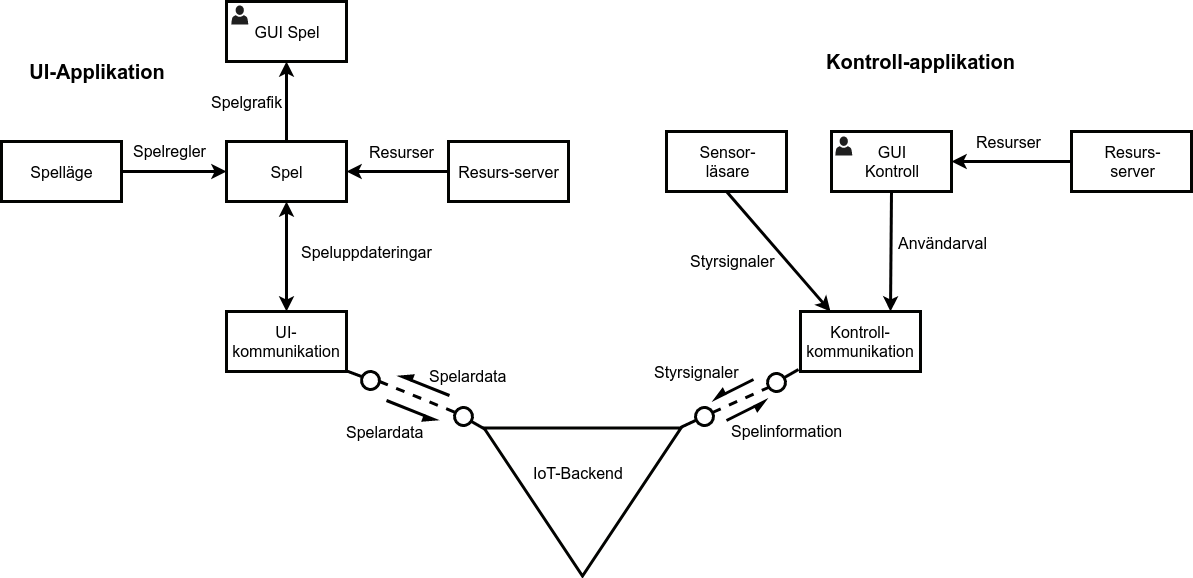
\includegraphics[scale=0.4]{konceptarkitektur}
    \caption{Modell över konceptarkitektur}
    \label{fig:konceptarkitektur}
\end{figure}

\subsubsection{Ansvarsområden}
\begin{labeling}{\small{\textbf{Kontrollkommunikation}}}
    \item [\small{\textbf{GUI Spel}}]
        \begin{itemize}
            \item Visa upp spelplanen
            \item Visa upp menyer
            \item Starta spel med specifika inställningar
            \newline
        \end{itemize}

    \item [\small{\textbf{Spelläge}}]
        \begin{itemize}
            \item Sätta upp regler för spelet
            \item Avgöra vilka resurser spelet ska innehålla
            \item Avgöra vad som ska ske vid olika tillfällen i spelet
            \newline
        \end{itemize}

    \item [\small{\textbf{Spel}}]
        \begin{itemize}
            \item Hålla koll på de olika spelarna
            \item Tillhandahålla grundläggande spelmekanik
            \newline
        \end{itemize}

    \item [\small{\textbf{Resursserver}}]
        \begin{itemize}
            \item Lagra vilka resurser som finns
            \item Ladda in resurser
            \newline
        \end{itemize}

    \item [\small{\textbf{UI-kommunikation}}]
        \begin{itemize}
            \item Upprätta uppkoppling mot server
            \item Förpacka data för kommunikation
            \newline
        \end{itemize}

    \item [\small{\textbf{Sensorläsare}}]
        \begin{itemize}
            \item Läsa av data från sensor
            \item Abstrahera sensordata till standardiserad form
            \item konfigurera sensor
            \newline
        \end{itemize}

    \item [\small{\textbf{GUI-kontroll}}]
        \begin{itemize}
            \item Visa menyer för att gå med i spelinstans
            \item Visa spelinformation om pågående spelet
            \item Tillhandahålla knappar på skärmen
            \newline
        \end{itemize}

    \item [\small{\textbf{Kontrollkommunikation}}]
        \begin{itemize}
            \item Upprätta uppkoppling mot server
            \item Förpacka data för kommunikation
            \newline
        \end{itemize}

    \item [\small{\textbf{IoT-Backend}}]
        \begin{itemize}
            \item Dirigera data mellan olika Kontroll-applikationer och olika instanser av UI-applikationen.
            \item Verifiera koder för att gå med i specifika spelinstanser.
            \newline
        \end{itemize}
\end{labeling}

\subsubsection{Beskrivning}
Arkitekturen är tydligt uppdelad i UI-applikation och kontroll-applikation. Från båda dessa finns specifika enheter som hanterar kommunikationen med den IoT-backend som är central i systemet. Dessa komponenters roll är att erbjuda ett gemensamt gränssnitt utåt för dataflöde. Då dessa två komponenter till stor del innehåller samma funktionalitet bör även delar av implementationen kunna återanvändas.\\

De två resursservrarna ska ses som instanser av samma komponent. Implementationen för dessa ska göras så pass generell att den kan användas både på UI- och kontroll-applikationen. En resursservers uppgift är att flytta ut arbetet med att ladda in resurser från implementationen i andra komponenter. I denna komponent finns också stora möjligheter att använda sig av cachning för Progressive Web Apps (referens?).\\

Spelläget är i denna modell en ensam komponent med endast ett gränssnitt mot den grundläggande spellogiken. Detta gränssnitt ska vara väldefinierat för att underlätta skapandet av nya spellägen. Med den nära kopplingen till resten av spelet finns också bra möjligheter till många kreativa spellägen, utan begränsing av omgivningen i systemet.\\

I arkitekturen för mobil-applikationen finns endast några få komponenter som uppfyller de nödvändiga kraven. Hela denna applikation får i denna struktur främst som uppgift att läsa data och skicka denna vidare. Detta är en lätt, icke prestandakrävande struktur.\\

Då arkitekturen inte består av många lager hålls datavägar genom den korta. Detta är centralt för responsivitet i en realtidsapplikation. Speciellt värt att notera är hur sensordata i kontroll-applikationen ej behöver passera fler komponenter för att nå applikationens kommunikations-gränssnitt.\\

Komponenten IoT-Backend är till viss del ett redan existerande system, men kommer att utökas med viss funktionalitet under projektet. I modellen är denna utökning ej separerad från resten av det systemet. Funktionalitet för att dirigera data kommer behöve skötas här för att tillåta flera olika instanser av UI-applikationen. Även all hantering av koder för anslutning till olika instanser bör därför implementeras i komponenten IoT-Backend.\\

				\subsection{Implementationsarkitektur}
Modell över implementationsarkitektur, koppling till motiveringen och diagram.

\subsubsection{Modell UI-Applikation}
Figur \ref{fig:implementationsarkitektur-UI} visar en modell över implementationsarkitekturen för UI-Applikationen. Kommunikationen från komponenten benämnd UI-kommunikation går till den IoT-Backend som presenteras i konceptarkitekturen.Denna är här utelämnad för tydlighet. Streckade rutor är grupperingar av komponenter som utgör stora delar i systemet. Gränssnittet mellan spel och spelläge ska betraktas som en viktig informationsväg och inte en självstående komponent.

\begin{figure}[h]
    \centering
    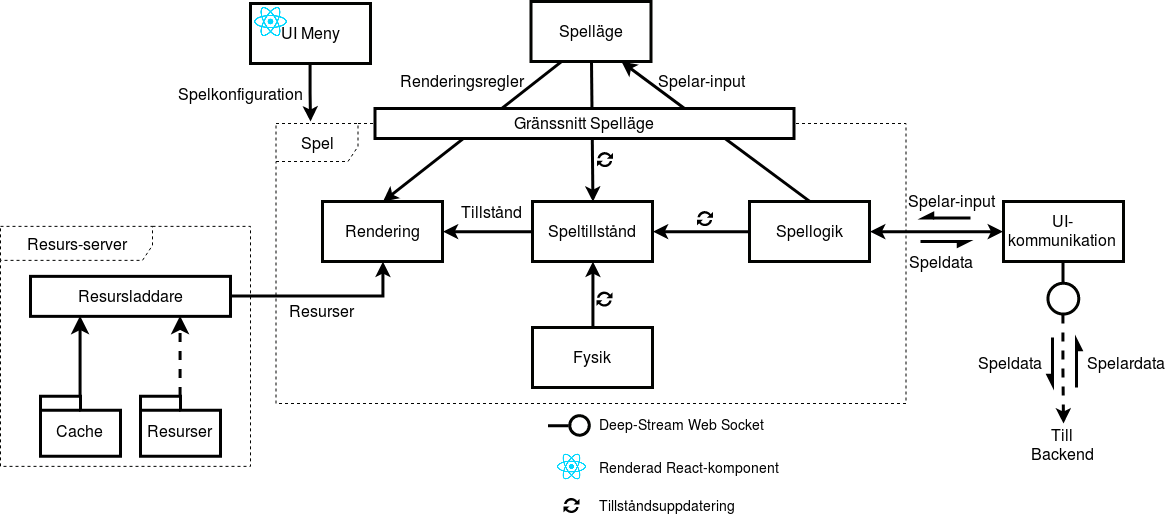
\includegraphics[scale=0.4]{implementationsarkitektur_UI}
    \caption{Modell över implementationsarkitektur för UI-Applikationen}
    \label{fig:implementationsarkitektur-UI}
\end{figure}

\subsubsection{Beskrivning UI-Applikation}

\subsubsection{Modell Kontroll-Applikation}
Implementationsarkitekturen för kontroll-applikationen presenteras i figur \ref{fig:implementationsarkitektur-kontroll}. Även denna följer samma notation som för UI-Applikationen. Resurs-servern är identisk med samma komponent i UI-delen.

\begin{figure}[h]
    \centering
    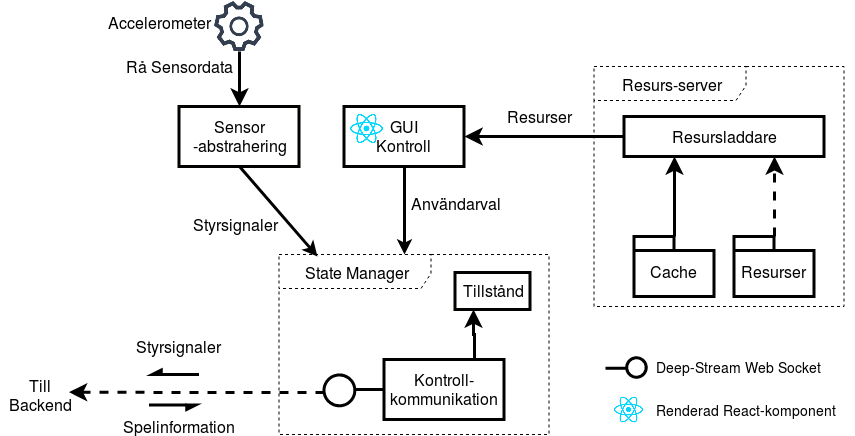
\includegraphics[scale=0.4]{implementationsarkitektur_kontroll}
    \caption{Modell över implementationsarkitektur för Kontroll-Applikationen}
    \label{fig:implementationsarkitektur-kontroll}
\end{figure}

\subsubsection{Beskrivning Kontroll-Applikation}

		\pagebreak

		\section{Diskussion}
Diskussion om möjliga problem med arkitektur och hur de kan bemötas. Idéer för framtida utökningar.

Arkitkturen lägger stor tilltro till att vissa komponenter klarar av uppgifter effektivt. Speciellt komponenten IoT-Backend är central för systemets responsivitet, då all data mellan Ui- och kontroll-applikation går genom denna. Här finns också begränsad möjlighet till optimering, då den till stor del består av ett redan existerande system som ej kan modifieras.\\

Det finns stora utmaningar gällande utformningen av gränssnittet mellan spellägen och spelet. Att få detta både väldefinierat och brett kräver en noggrann och välgrundad design. Detta kan underlättas då man får en bättre bild av spellägen som ska implementeras.\\

Arkitekturens användargränssnitt har fler ansvarsområden än att endast visa upp saker. Detta gäller främst logik som ligger nära utritning av grafik och menyer. Om denna logik inte växer alltför mycket och kräver interaktion med fler komponenter bör detta ej bli ett problem. Det går dock att bryta ut denna logik i framtiden till en egen komponent.\\

Spelets kontroller i kontroll-applikationen kan i framtiden generellaiseras. För att tillåta andra styrningsmetoder än sensorer kan flera komponenter behöva skapas. Dessa bör struktureras så att oavsett hur användaren kontrollerar spelet blir den slutgilitga datan som skickas till UI-komponenten densamma.

		\pagebreak

    \printbibliography
    \pagebreak

		\begin{appendices}
				\section{Use case maps konceptarkitektur}

\begin{figure}[h]
    \centering
    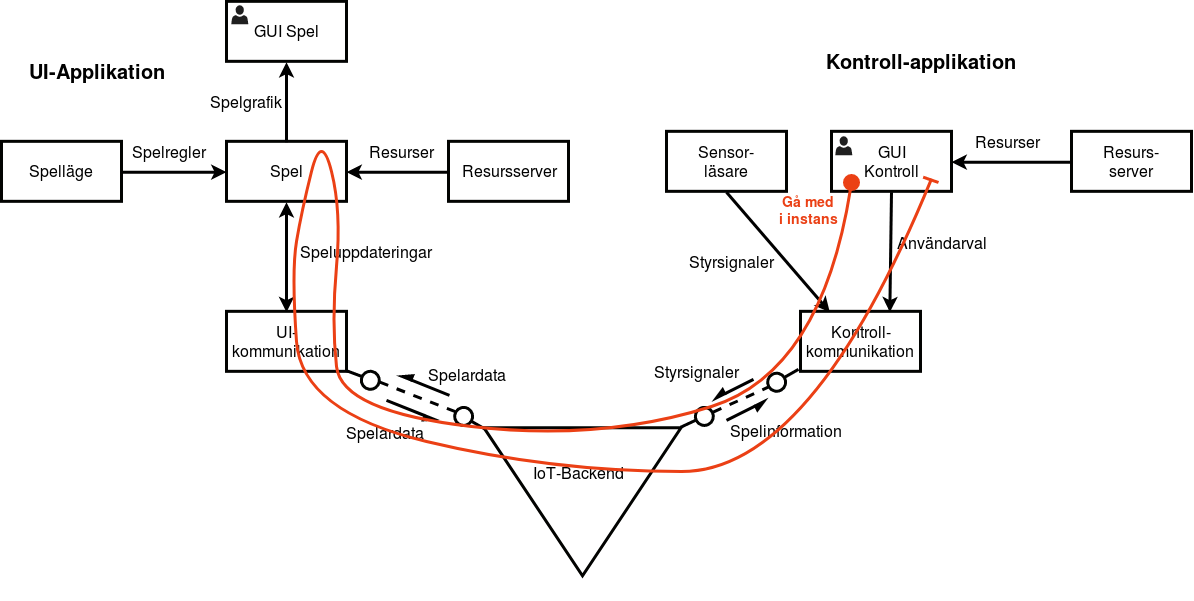
\includegraphics[scale=0.4]{konceptuell_use_case_join_instans}
    \caption{Use case map för att gå med i instans}
    \label{fig:use_case_koncept_join}
\end{figure}

\begin{figure}[h]
    \centering
    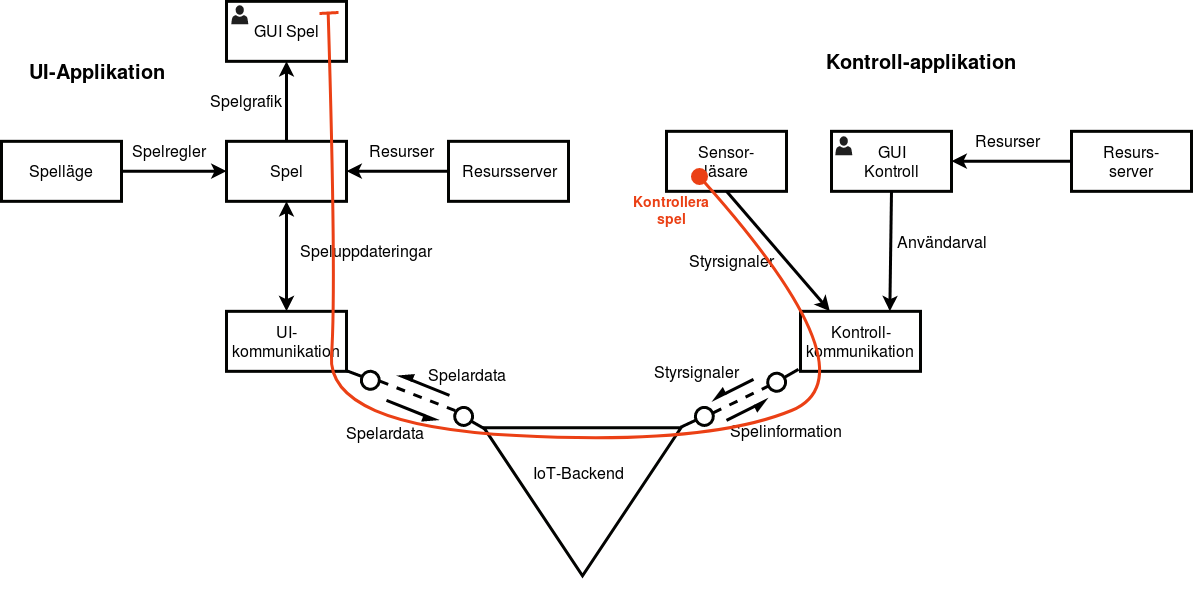
\includegraphics[scale=0.4]{konceptuell_use_case_kontrollera_spel}
    \caption{Use case map för att kontrollera spelet}
    \label{fig:use_case_koncept_kontrollera}
\end{figure}

\begin{figure}[h]
    \centering
    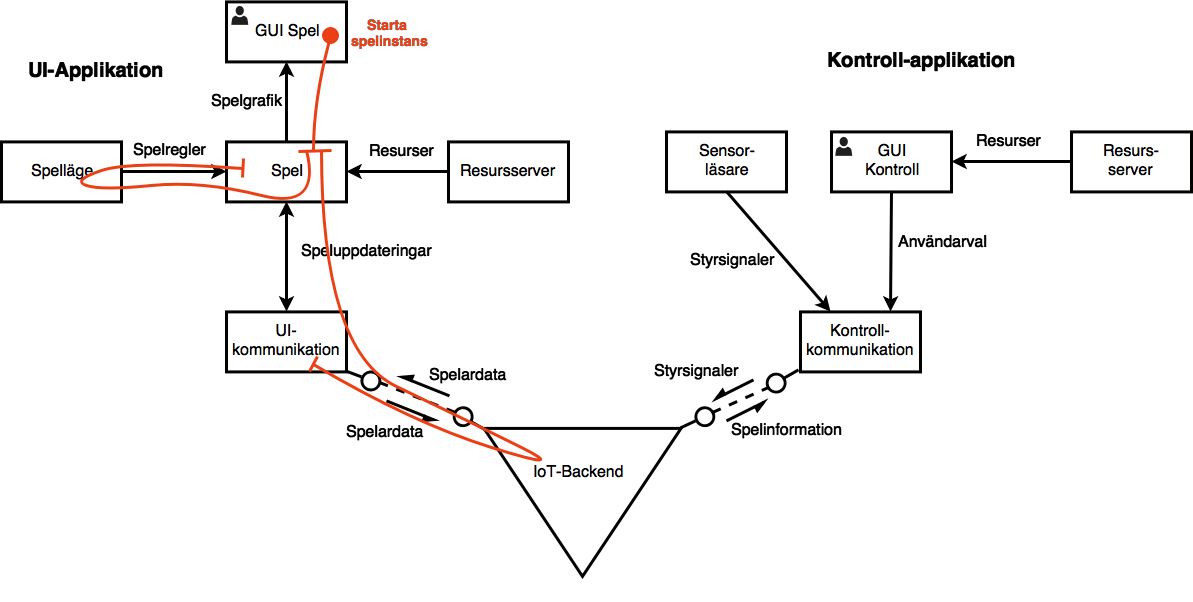
\includegraphics[scale=0.4]{konceptuell_use_case_starta_spelinstans}
    \caption{Use case map för att starta en spelinstans}
    \label{fig:use_case_koncept_starta_instans}
\end{figure}

\begin{figure}[h]
    \centering
    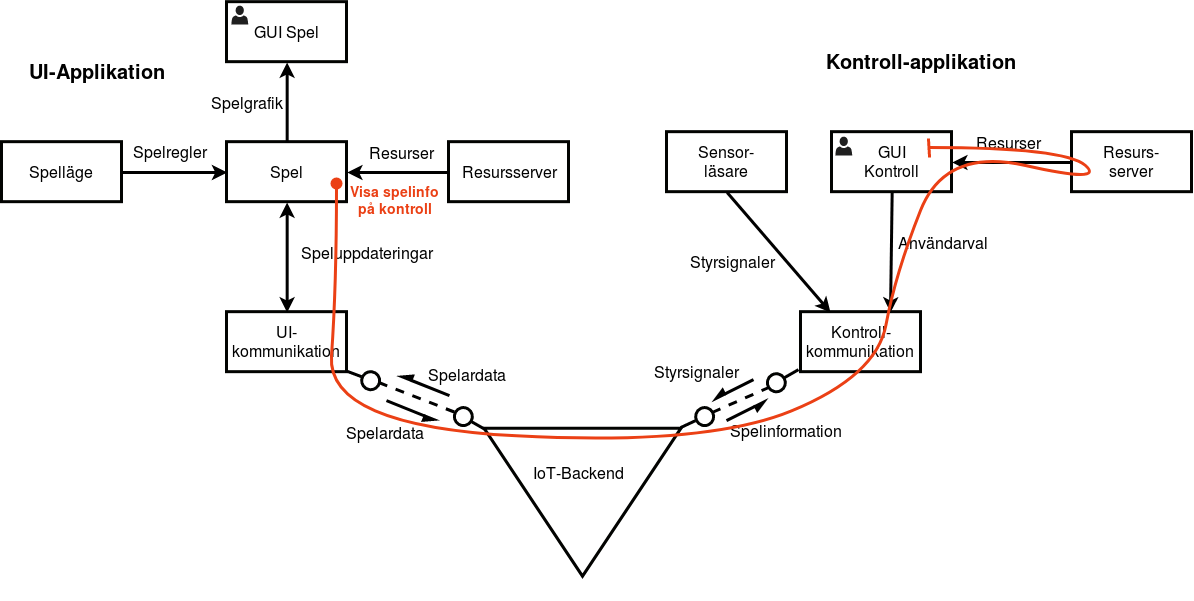
\includegraphics[scale=0.4]{images/konceptuell_use_case_visa_spelinfo}
    \caption{Use case map för att visa upp spelinformation i kontroll-applikationen}
    \label{fig:use_case_koncept_visa_spelinfo}
\end{figure}

\begin{figure}[h]
    \centering
    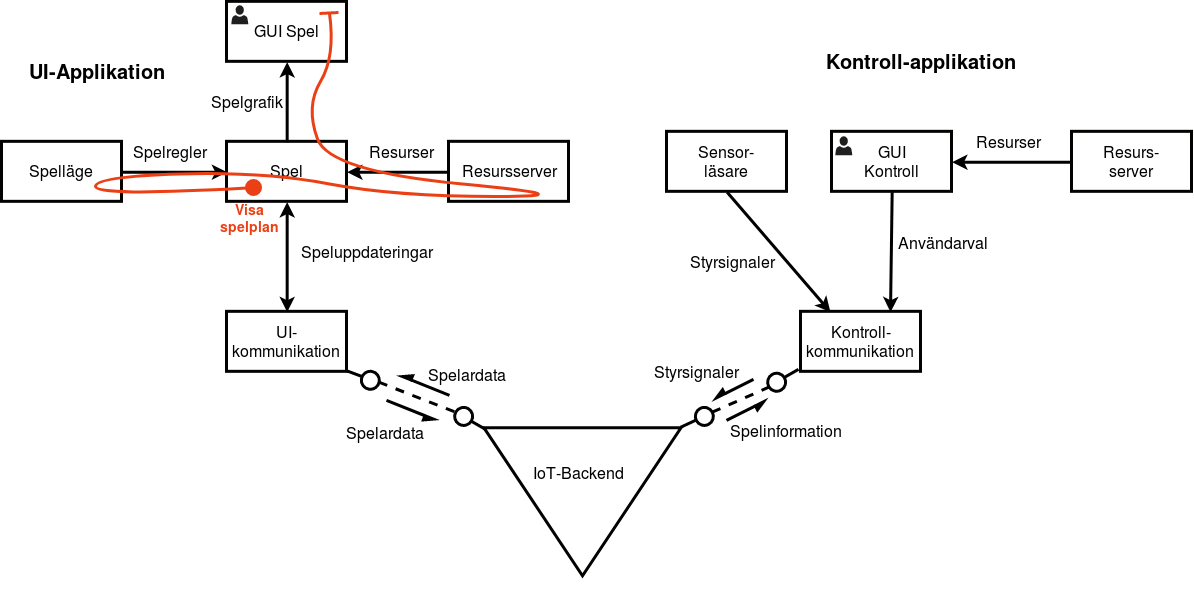
\includegraphics[scale=0.4]{images/konceptuell_use_case_visa_spelplan}
    \caption{Use case map för att visa upp spelplanen i UI-applikationen}
    \label{fig:use_case_koncept_visa_spelplan}
\end{figure}

        \pagebreak
        \section{Use case maps för implementationsarkitektur}
\label{sec:use_case_implementation}

\begin{figure}[h]
    \centering
    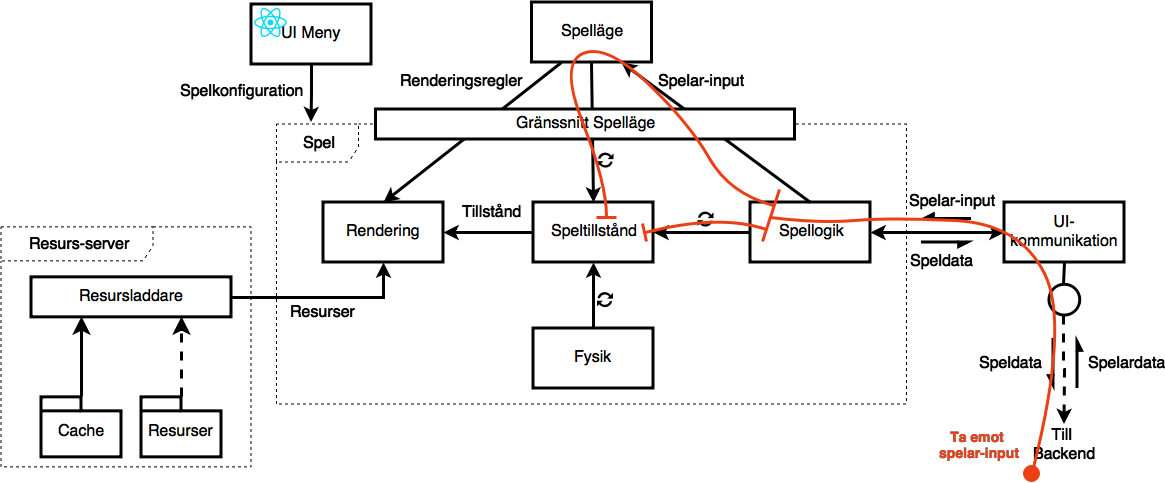
\includegraphics[scale=0.4]{implementation_use_case_ta_input}
    \caption{Use case map för att ta emot spelar-input}
    \label{fig:use_case_implementation_input}
\end{figure}

\begin{figure}[h]
    \centering
    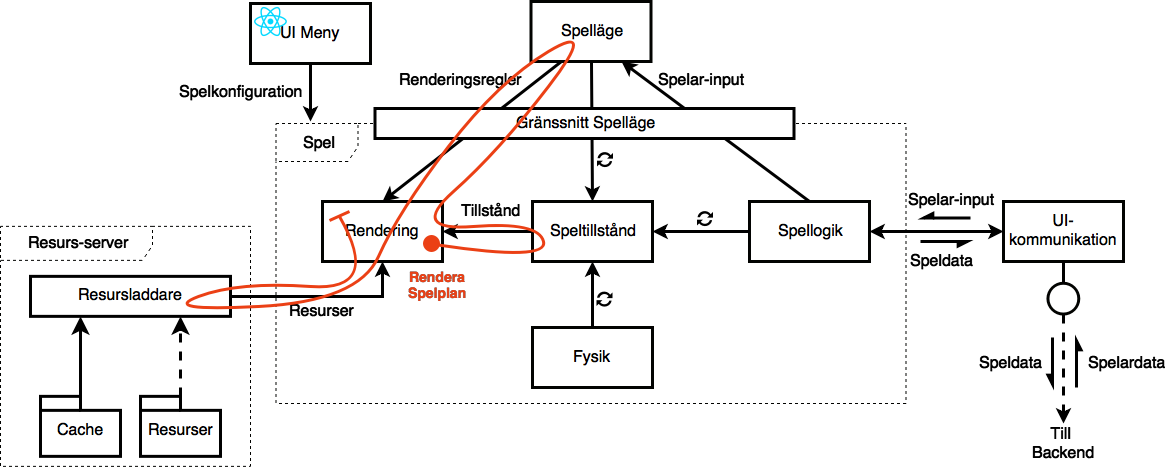
\includegraphics[scale=0.4]{implementation_use_case_rendera_spelplan}
    \caption{Use case map för att rendera spelplanen}
    \label{fig:use_case_implementation_rendera}
\end{figure}

\pagebreak

\section{Impact maps för implementationsarkitektur}
\label{sec:impact_implementation}

\begin{figure}[h]
    \centering
    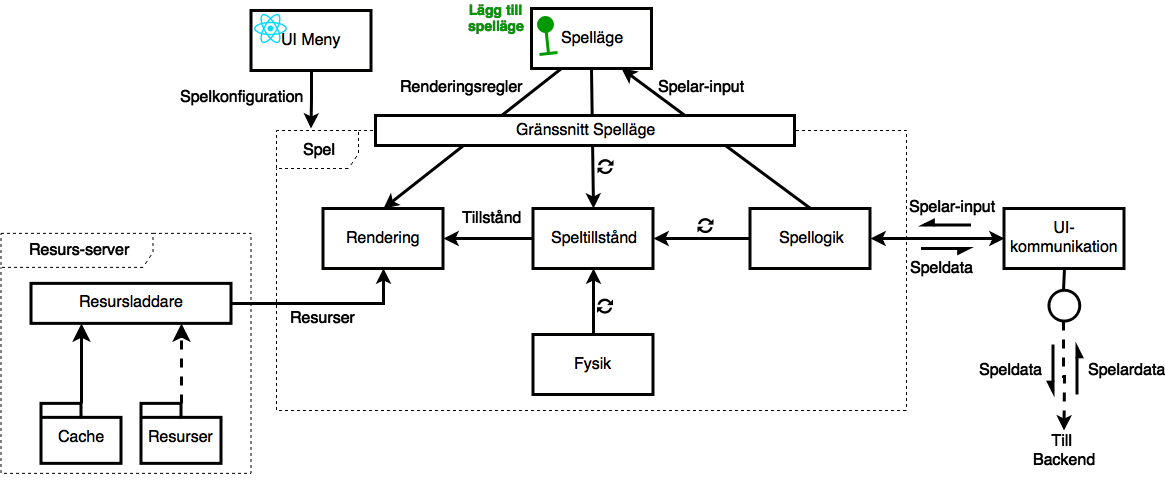
\includegraphics[scale=0.4]{implementation_impact_nytt_spellage}
    \caption{Impact map för att lägga till ett nytt spelläge}
    \label{fig:impact_implementation_spellage}
\end{figure}

\begin{figure}[h]
    \centering
    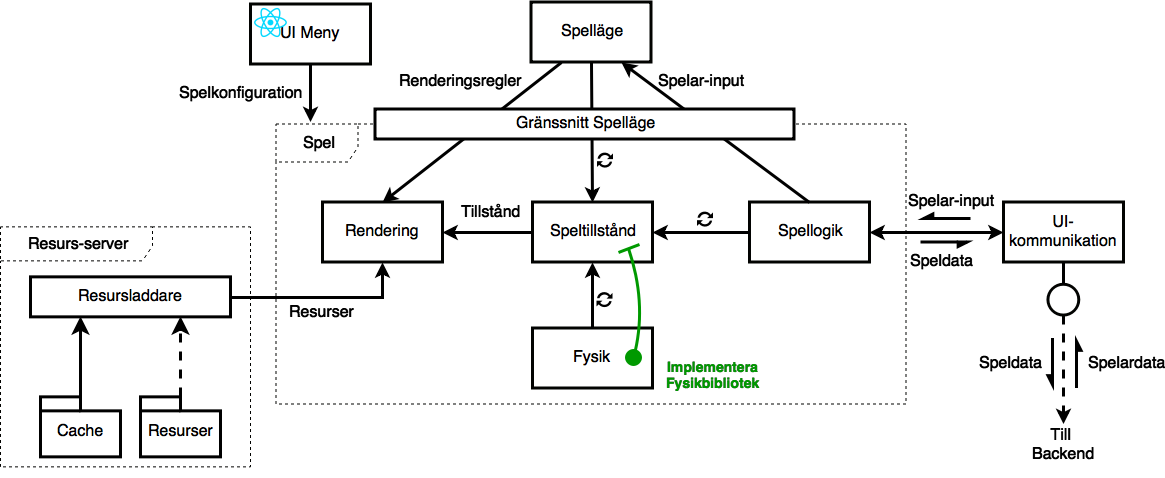
\includegraphics[scale=0.4]{implementation_impact_fysikbibliotek}
    \caption{Impact map för att implementera ett färdigt fysikbibliotek}
    \label{fig:impact_implementation_fysikbibliotek}
\end{figure}

\begin{figure}[h]
    \centering
    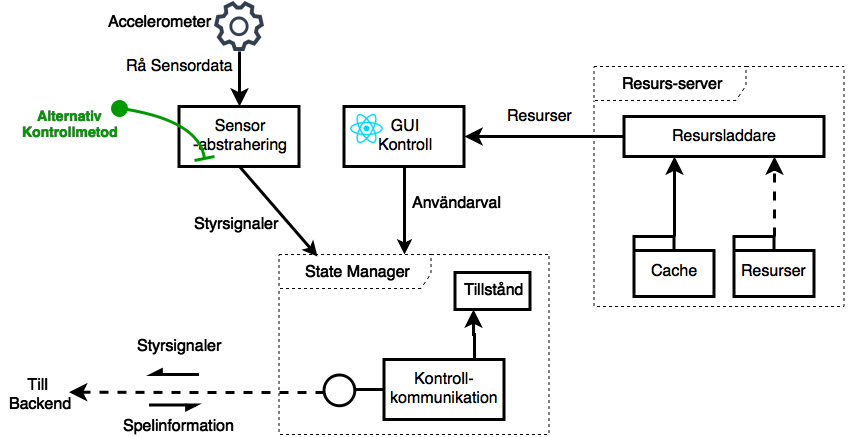
\includegraphics[scale=0.4]{implementation_impact_alternativ_kontroll}
    \caption{Impact map för att lägga till en alternativ kontrollmetod}
    \label{fig:impact_implementation_alt_kontroll}
\end{figure}

		\end{appendices}
\end{document}
